\chapter{Введение}

\section{Актуальность темы исследования}

Текст актуальности исследования. Здесь необходимо обосновать важность выбранной темы, показать её значимость для науки и практики. Современные исследования в области искусственного интеллекта \cite{ai_survey} показывают значительный прогресс в разработке новых алгоритмов и методов.

\begin{figure}[H]
\centering
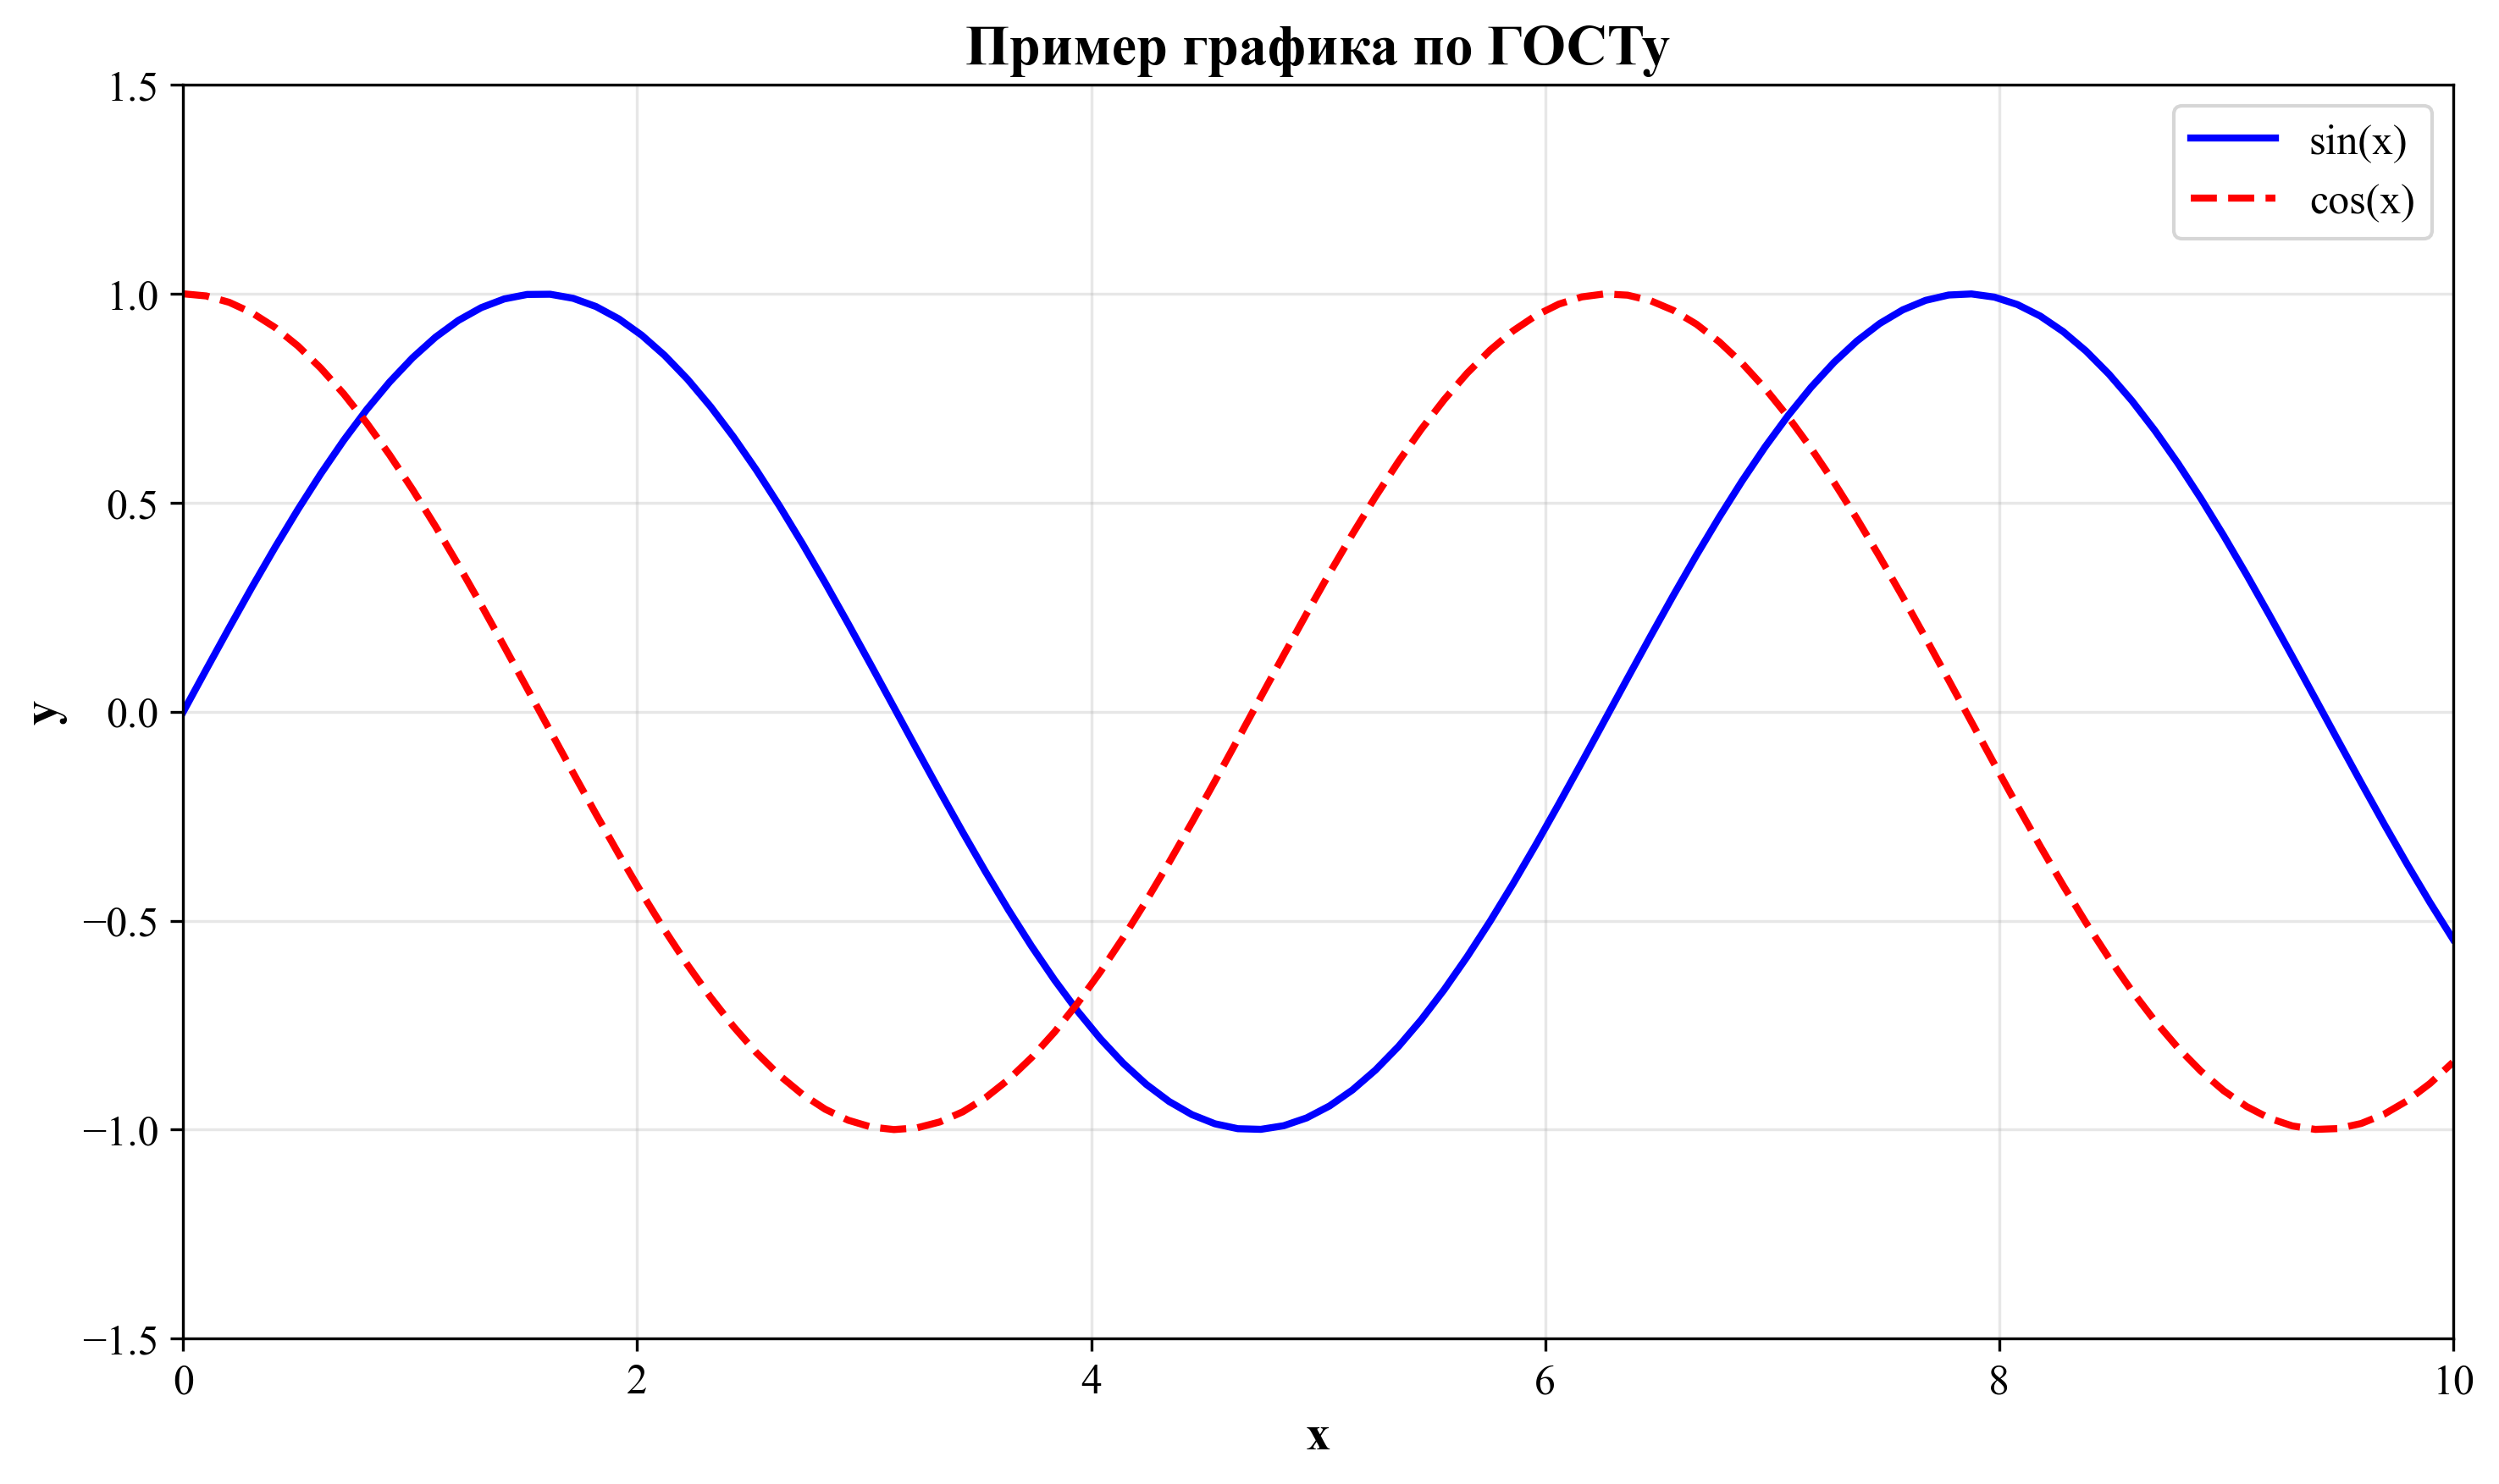
\includegraphics[width=0.7\textwidth]{images/example_plot.png}
\caption{Рост интереса к машинному обучению за последние годы}
\label{fig:ml_growth}
\end{figure}

На рисунке \ref{fig:ml_growth} показан рост интереса к технологиям машинного обучения, что подтверждает актуальность выбранной темы исследования.

\begin{table}[H]
\centering
\caption{Статистика использования ИИ в различных отраслях}
\label{tab:ai_usage_stats}
\begin{tabular}{|l|c|c|}
\hline
\textbf{Отрасль} & \textbf{Проникновение ИИ} & \textbf{Рост за год} \\
\hline
Здравоохранение & 45\% & +15\% \\
Финансы & 60\% & +12\% \\
Транспорт & 35\% & +20\% \\
Образование & 25\% & +18\% \\
\hline
\end{tabular}
\end{table}

В таблице \ref{tab:ai_usage_stats} представлена статистика внедрения технологий искусственного интеллекта в различных отраслях экономики.

\begin{equation}
L(\theta) = \frac{1}{m} \sum_{i=1}^{m} \log p(y^{(i)} | x^{(i)}; \theta)
\label{eq:log_likelihood}
\end{equation}

Формула \ref{eq:log_likelihood} описывает функцию логарифмического правдоподобия, используемую в машинном обучении для оценки качества модели.

\begin{CodeBlock}{Python}{Пример анализа данных}{lst:data_analysis}
import pandas as pd
import matplotlib.pyplot as plt

# Load and analyze data
data = pd.read_csv('research_data.csv')
print("Dataset size: %s" % str(data.shape))
print("Missing values: %d" % data.isnull().sum().sum())

# Visualize distribution
plt.figure(figsize=(10, 6))
data['target'].hist(bins=30)
plt.title('Target variable distribution')
plt.xlabel('Value')
plt.ylabel('Frequency')
plt.show()
\end{CodeBlock}

В листинге \ref{lst:data_analysis} показан пример анализа данных для исследования, демонстрирующий современные подходы к обработке информации.

\section{Степень разработанности проблемы}

Анализ существующих исследований по теме. Обзор работ отечественных и зарубежных авторов.

\section{Цель и задачи исследования}

\subsection{Цель исследования}

Сформулировать основную цель работы.

\subsection{Задачи исследования}

\begin{enumerate}
    \item Первая задача;
    \item Вторая задача;
    \item Третья задача;
    \item И так далее.
\end{enumerate}

\section{Объект и предмет исследования}

\subsection{Объект исследования}

Описание объекта исследования.

\subsection{Предмет исследования}

Описание предмета исследования.

\section{Методы исследования}

Перечисление методов, используемых в работе.

\section{Научная новизна}

Описание научной новизны исследования.

\section{Практическая значимость}

Описание практической значимости результатов работы.

\section{Структура работы}

Краткое описание структуры диссертации с указанием количества страниц в каждой главе.

\section{Апробация результатов}

Информация о публикациях, выступлениях на конференциях и других формах апробации результатов.
